\section{Ordinary Differential Equations}
\subsection{Euler's Method}
The general form of a first order one variable ODE is:
$$\dfrac{dx}{dt}=f(x,t)$$
We begin with an initial value condition, say $x = a$ at $t=0 $. We then calculate $x$ at $t+h$ given by $x(t+h)= x(t)+dx$, where $dx$ is obtained by equation $$dx=dt*(f(x(t), t))$$ Accordingly, $dt = h$, where $$h=\dfrac{t_{max}-t_{min}}{N},$$where $N$ is the number of steps we choose to have.
This is known as Euler's Method.
\begin{lstlisting}[language=Python, caption=Euler's Method, frame=single, label={lst:euler} ]
def f(x,t):
	return -x**3+np.sin(t)
N=1000
tval=np.linspace(0,10,N)
x=0
xval=[]
a=tval[0]
b=tval[N-1]
h=(b-a)/N
for t in tval:
	xval.append(x)
	x+=h*f(x,t)
plt.plot(tval,xval)
plt.title('$\dfrac{dx}{dt}=-x^{3}+\sin{(x)}$')
\end{lstlisting}
\begin{figure}[H]
	\centering
	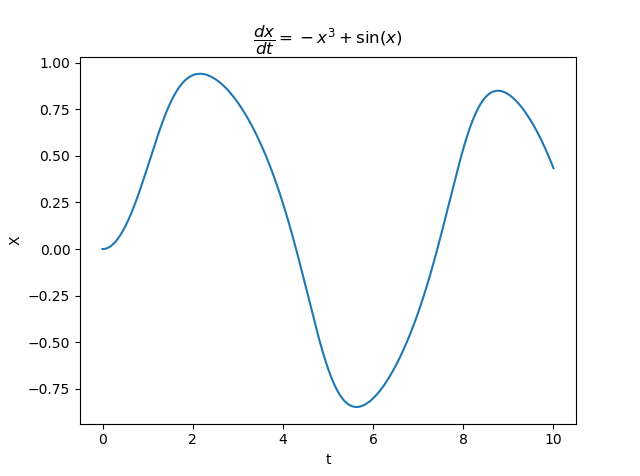
\includegraphics[width=0.7\linewidth]{Euler'sMethod}
	\caption{$x(t), t\in(0,10)$}
	\label{fig:eulersmethod}
\end{figure}
\newpage
\subsection{Runge-Kutta Method (RK4)}
Let,
$$k_{1}=hf(x,t)$$$$k_{2}=hf(x+\dfrac{k_{1}}{2}, t+\dfrac{h}{2})$$$$k_{3}=hf(x+\dfrac{k_{2}}{2}, t+\dfrac{h}{2})$$$$k_{4}=hf(x+k_{3}, t+h),$$then, we have:
$$x(t+h)=x(t)+\dfrac{(k_{1}+2k_{2}+2k_{3}+k_{4})}{6}$$
This is the \textbf{Fourth-Order Runge-Kutta Method}. \\
\textbf{Implementation:}
\begin{lstlisting}[language=Python, caption=RK4 Method, frame=single, label={lst:RK4} ]
for N in [10,20,50,100]:
	tval=np.linspace(0,10,N)
	a=tval.min()
	b=tval.max()
	h=(b-a)/N
	x=0
	xval=[]
	for t in tval:
		k1=h*f(x,t)
		k2=h*f(x+k1/2,t+h/2)
		k3=h*f(x+k2/2,t+h/2)
		k4=h*f(x+k3,t+h)
		x+=1/6*(k1+2*k2+2*k3+k4)
		xval.append(x)
	plt.plot(tval,xval,label=f"N={N}")

\end{lstlisting}
\begin{figure}[H]
	\centering
	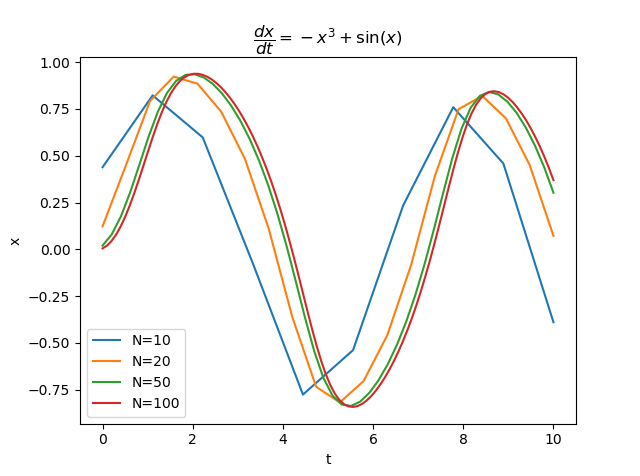
\includegraphics[width=0.7\linewidth]{RK4}
	\caption{RK4 Method}
	\label{fig:rk4}
\end{figure}

\subsection{Simultaneous Ordinary Differential Equations}
Let,$$\dfrac{dx}{dt}=f_{x}(x,y,t)$$\\ $$\dfrac{dy}{dt}=f_{y}(x,y,t)$$They can be re-written into vector notation as: $$\dfrac{d\textbf{r}}{dt}=\textbf{f}(\textbf{r}, t)$$ Therefore,$$\textbf{r}(t+h)=\textbf{r}(t)+h\textbf{f}(\textbf{r},t)$$ \\
Further Taylor Expansions used to derive Runge-Kutta rules also generalize straightforwardly to the multi-variable case. Thus, $$\textbf{r}(t+h)=\textbf{r}(t)+\dfrac{\textbf{$k_{1}$}+2(\textbf{$k_{2}+k_{3}$})+k_{4}}{6}$$
\subsubsection{The Lorenz Equations}
The Lorenz Equations are:
$$\dfrac{dx}{dt}=\sigma(y-x)$$$$\dfrac{dy}{dt}=rx-y-xz$$$$\dfrac{dz}{dt}=xy-bz$$
To Plot:
\begin{lstlisting}[language=Python, caption=Lorenz Plotter, frame=single, label={lst:Lorenz} ]
s=np.float64(10.0)
r=np.float64(28.0)
b=np.float64(8/3)
def f(R):
	x=R[0]
	y=R[1]
	z=R[2]
	fx=s*(y-x)
	fy=r*x-y-x*z
	fz=x*y-b*z
	return np.float64([fx,fy,fz])
tmin=np.float64(0)
tmax=np.float64(35)
N=3000
h=(tmax-tmin)/N
tval=np.linspace(tmin,tmax,N)
R=np.float64([0,1,0])
xval=[]
yval=[]
zval=[]
for t in tval:
	k1=h*f(R)
	k2=h*f(R+h/2)
	k3=h*f(R+k2/2)
	k4=h*f(R+k3)
	R+=(k1+2*k2+2*k3+k4)/6
	xval.append(R[0])
	yval.append(R[1])
	zval.append(R[2])
ax = plt.axes(projection='3d')
ax.plot3D(xval, yval, zval, color="Blue")

\end{lstlisting}
\begin{figure}[H]
	\centering
	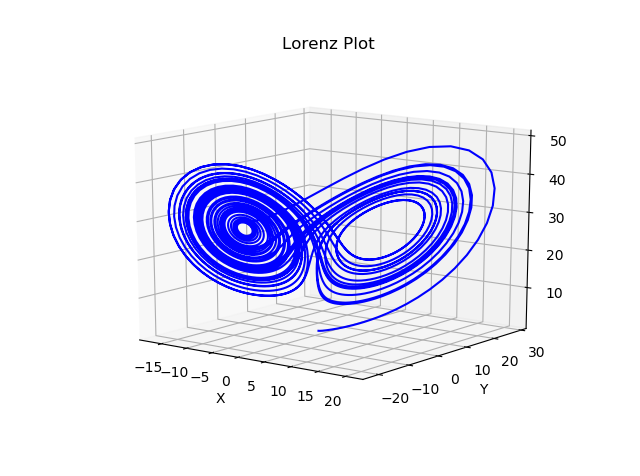
\includegraphics[width=0.9\linewidth]{LorenzPlot}
	\caption{Lorenz Plot}
	\label{fig:lorenzplot}
\end{figure}


